\documentclass[11pt,a4paper]{article}
\usepackage[utf8]{inputenc}
\usepackage[T1]{fontenc}
\usepackage{geometry}
\geometry{margin=2.4cm}
\usepackage{xcolor}
\usepackage{tikz}
\usetikzlibrary{arrows.meta, positioning, fit, calc, backgrounds}
\usepackage{booktabs}
\usepackage{tabularx}
\usepackage{enumitem}
\usepackage{hyperref}
\usepackage{fancyhdr}
\usepackage{titlesec}
\usepackage{tcolorbox}
\tcbuselibrary{skins, breakable}
\usepackage{float}
\usepackage{eurosym}

% Colours
\definecolor{sub}{RGB}{30, 60, 114}
\definecolor{acc}{RGB}{190, 60, 50}
\definecolor{grn}{RGB}{46, 139, 87}

% Header
\pagestyle{fancy}
\fancyhf{}
\fancyhead[L]{\small\textcolor{sub}{\textbf{Substrate House}}}
\fancyhead[R]{\small\textcolor{sub}{Proposal A}}
\fancyfoot[C]{\thepage}
\renewcommand{\headrulewidth}{0.4pt}
\renewcommand{\headrule}{\hbox to\headwidth{\color{sub}\leaders\hrule height \headrulewidth\hfill}}

\titleformat{\section}{\large\bfseries\color{sub}}{\thesection}{1em}{}[\vspace{-0.5em}\textcolor{sub}{\rule{\textwidth}{0.3pt}}]
\titleformat{\subsection}{\normalsize\bfseries\color{sub!80}}{\thesubsection}{1em}{}

\setlength{\parskip}{0.45em}
\setlength{\parindent}{0pt}

\title{%
  \textcolor{sub}{\rule{\textwidth}{1.2pt}}\\[0.4cm]
  {\LARGE\bfseries\textcolor{sub}{Soba}}\\[0.1cm]
  {\large\textcolor{sub!60}{A humanoid robot that feels what you feel}}\\[0.3cm]
  \textcolor{sub}{\rule{\textwidth}{1.2pt}}
}
\author{\textbf{Substrate House} \textperiodcentered\ London}
\date{April 2026}

\begin{document}
\maketitle
\thispagestyle{fancy}

% ──────────────────────────────────────────────────────────────────────────────
\section{The idea}

We want to put a person in a room with a robot, wire the person up with EEG, ECG, and eye tracking, and have the robot \emph{know} --- in real time --- whether that person is stressed, focused, zoning out, overloaded, or in flow. And then have the robot change what it's doing accordingly.

Not in the way a chatbot changes its tone. Physically. The robot slows its walk, opens its palms, steps back, lowers its posture. Or it leans in, gestures, steps closer. The adaptation is embodied, legible, and immediate --- within half a second of a state change in the person's nervous system.

We call the robot \textbf{Soba}. This proposal describes building it as a humanoid.

% ──────────────────────────────────────────────────────────────────────────────
\section{Why it has to be a body}

The existing literature on biosignal-adaptive HRI is almost entirely screen-based or limited to facial display robots~\cite{szafir2012, kulic2007}. Szafir and Mutlu's work showed that a NAO robot adapting verbal cues to EEG-measured attention improved recall by 43\% --- but the robot's physical behaviour was barely used. Kuli\'{c} and Croft demonstrated real-time affective estimation from GSR and heart rate, but only applied it to trajectory planning for an industrial arm.

Nobody has closed the full loop: continuous multimodal biosignal inference driving whole-body humanoid behaviour in real time. That's what we're building.

The humanoid form matters because the output space is richer than any alternative. A wheeled robot with an LCD face can only vary speed and screen graphics. A humanoid can vary posture (open vs.\ closed), gait (fast, slow, hesitant), gesture (palms up, pointing, still), proximity (approach, retreat), head orientation (tracking, averted), and overall body tension --- all channels that humans decode without conscious effort. We are building a robot that speaks body language, and body language requires a body.

The risk is the uncanny valley. A humanoid that adapts \emph{almost} correctly might feel worse than a screen that gets it wrong. We think the answer is to keep the movements slow, smooth, and slightly stylised rather than attempting photorealism. More like a mime than a mannequin.

% ──────────────────────────────────────────────────────────────────────────────
\section{Architecture}

\begin{figure}[H]
\centering
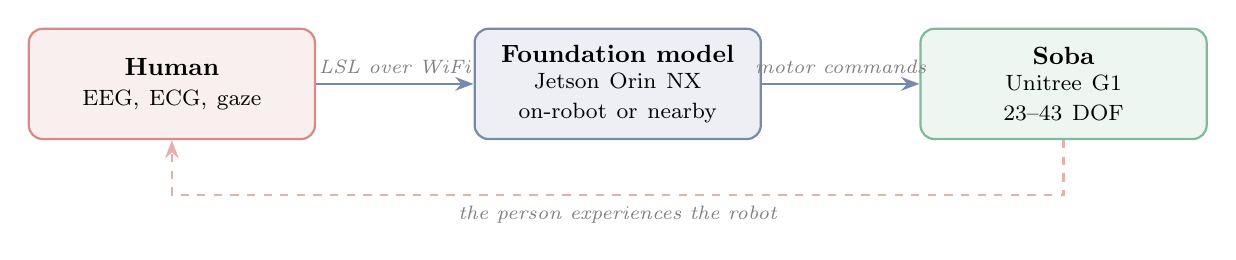
\begin{tikzpicture}[
    >=Stealth, node distance=1.2cm,
    block/.style={rectangle, rounded corners=5pt, draw=#1!60, fill=#1!8,
      text width=3.4cm, minimum height=1.4cm, align=center,
      font=\small\bfseries, line width=0.8pt},
    arr/.style={->, thick, sub!60},
    lbl/.style={font=\scriptsize\itshape, text=gray}
  ]
  \node[block=acc] (human) {Human\\{\footnotesize\normalfont EEG, ECG, gaze}};
  \node[block=sub, right=2cm of human] (compute) {Foundation model\\{\footnotesize\normalfont Jetson Orin NX\\on-robot or nearby}};
  \node[block=grn, right=2cm of compute] (robot) {Soba\\{\footnotesize\normalfont Unitree G1\\23--43 DOF}};
  \draw[arr] (human) -- node[above, lbl]{LSL over WiFi} (compute);
  \draw[arr] (compute) -- node[above, lbl]{motor commands} (robot);
  \draw[arr, dashed, acc!40] (robot.south) -- ++(0,-0.7) -| node[below, pos=0.25, lbl]{the person experiences the robot} (human.south);
\end{tikzpicture}
\caption{The loop. Biosignals flow from the person to the model; the model's state vector drives the robot's body; the robot's body changes how the person feels, which changes the biosignals. This is a closed physiological--behavioural loop.}
\label{fig:arch}
\end{figure}

The interesting part of this diagram is the dashed line at the bottom. This is not a one-shot classification problem. The robot's behaviour feeds back into the person's physiology. If Soba detects high stress and responds by slowing down and stepping back, we should see the stress signal drop --- and then Soba can gradually re-engage. The system is a dynamical loop, not a pipeline. Our behaviour policy needs to account for this; naive threshold-based switching will oscillate.

% ──────────────────────────────────────────────────────────────────────────────
\section{The robot}

We are using the \textbf{Unitree G1} in its EDU configuration. A year ago this would have been impossible without a six-figure budget; the G1 changed the economics of humanoid research.

\begin{table}[H]
\centering\small
\begin{tabularx}{\textwidth}{lX}
\toprule
Height / Weight & 1.32\,m, 35\,kg --- roughly the size of a 9-year-old \\
Degrees of freedom & 23 (base) to 43 (EDU + Dex3-1 hands) \\
Onboard compute & NVIDIA Jetson Orin \\
Sensors & 3D LiDAR, depth cameras, IMU \\
Battery life & $\sim$2\,h on a 9\,Ah quick-release pack \\
SDK & Python, ROS2 \\
Price & \$18k--\$25k depending on configuration \\
\bottomrule
\end{tabularx}
\caption*{Unitree G1 EDU --- \url{https://shop.unitree.com/products/unitree-g1}}
\end{table}

We want the EDU variant specifically because it ships with the Jetson Orin, which gives us enough compute to run a moderate foundation model directly on the robot. If the model turns out to be too large, we offload inference to a companion \href{https://www.seeedstudio.com/reComputer-J4012-p-5586.html}{Seeed reComputer J4012} (Jetson Orin NX 16\,GB, \$1,099) communicating over a dedicated 5\,GHz WiFi link. We design the software to support both from day one --- it's just a flag in the inference node config.

The G1's SDK is still young. We expect to spend real engineering time on low-level motor APIs for expressive gesture. This is a known cost of being early.

% ──────────────────────────────────────────────────────────────────────────────
\section{What the person wears}

We want the lightest possible sensor load that still gives us the signals we need. Every additional wire or strap increases participant burden and changes the behaviour we're trying to study.

\begin{table}[H]
\centering\small
\begin{tabularx}{\textwidth}{llXr}
\toprule
\textbf{Signal} & \textbf{Device} & \textbf{What we get from it} & \textbf{Price} \\
\midrule
EEG & \href{https://mbraintrain.com/smarting-pro/}{mBrainTrain Smarting PRO} & Neural oscillations, cognitive load, attention, arousal at ms resolution. 24 channels, wireless, streams directly to LSL. & \euro 15k \\
Eye tracking & \href{https://pupil-labs.com/products/neon}{Pupil Labs Neon} & Gaze direction, fixation, saccades, pupil dilation (arousal/load proxy), blink rate. & \euro 4.5k \\
ECG & \href{https://www.polar.com/uk-en/sensors/h10-heart-rate-sensor}{Polar H10} & Heart rate variability --- the cleanest peripheral readout of autonomic balance we can get from a \pounds 70 chest strap. RMSSD and LF/HF ratio give us stress and recovery state on a seconds-to-minutes timescale. & \pounds 70 \\
EDA & \href{https://shimmersensing.com/product/shimmer3-gsr-unit/}{Shimmer3 GSR+} & Electrodermal activity. Purely sympathetic signal --- an unambiguous stress/arousal marker that complements pupil dilation (which is contaminated by luminance). & \euro 1.2k \\
\bottomrule
\end{tabularx}
\end{table}

We already own EEG and eye tracking equipment. The ECG and EDA sensors are new additions to our setup. The ECG in particular fills a gap: our current recording configurations have no direct autonomic measure, and autonomic state is arguably the most actionable signal for robot behaviour modulation.

% ──────────────────────────────────────────────────────────────────────────────
\section{The model and the pipeline}

All sensors stream to a single receiver via Lab Streaming Layer (LSL) over WiFi. LSL handles cross-device clock synchronisation, which is non-trivial when EEG runs at 250\,Hz, eye tracking at 120\,Hz, ECG at 130\,Hz, and EDA at 64\,Hz.

The preprocessing node applies per-modality filtering (bandpass 1--45\,Hz and 50\,Hz notch for EEG; modified Beer-Lambert for fNIRS if present; HRV feature extraction for ECG), then windows everything into aligned 500\,ms segments sliding by 100\,ms. This gives us a 10\,Hz update rate into the model.

The foundation model takes the windowed multimodal tensor and outputs a state vector: a continuous representation of cognitive load, arousal, stress, attention, and flow. We export the model to TensorRT with FP16 quantisation for Jetson deployment. Target inference latency is under 200\,ms.

\begin{figure}[H]
\centering
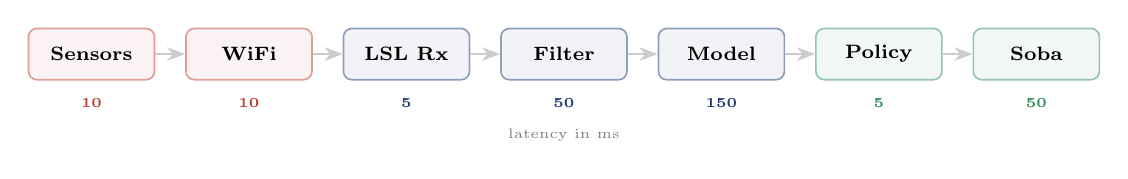
\begin{tikzpicture}[
    >=Stealth,
    box/.style={rectangle, rounded corners=3pt, draw=#1!50, fill=#1!6,
      minimum width=1.6cm, minimum height=0.65cm, align=center,
      font=\scriptsize\bfseries, line width=0.6pt},
    time/.style={font=\tiny\bfseries, text=#1}
  ]
  \node[box=acc] (s1) at (0,0) {Sensors};
  \node[box=acc] (s2) at (2,0) {WiFi};
  \node[box=sub] (s3) at (4,0) {LSL Rx};
  \node[box=sub] (s4) at (6,0) {Filter};
  \node[box=sub] (s5) at (8,0) {Model};
  \node[box=grn] (s6) at (10,0) {Policy};
  \node[box=grn] (s7) at (12,0) {Soba};
  \foreach \a/\b in {s1/s2, s2/s3, s3/s4, s4/s5, s5/s6, s6/s7} {
    \draw[->, gray!40, thick] (\a.east) -- (\b.west);
  }
  \node[time=acc, below=3pt of s1] {10};
  \node[time=acc, below=3pt of s2] {10};
  \node[time=sub, below=3pt of s3] {5};
  \node[time=sub, below=3pt of s4] {50};
  \node[time=sub, below=3pt of s5] {150};
  \node[time=grn, below=3pt of s6] {5};
  \node[time=grn, below=3pt of s7] {50};
  \node[font=\tiny, text=gray, below=14pt of s4] {latency in ms};
\end{tikzpicture}
\caption{End-to-end latency: $\sim$280\,ms. We need to be under 500\,ms. Behavioural adaptation operates on a seconds timescale in human perception, so this is comfortable.}
\end{figure}

% ──────────────────────────────────────────────────────────────────────────────
\section{How Soba behaves}

The behaviour policy is the part of this project that will take the most iteration and is hardest to get right on paper. The table below is our starting point, not a finished design.

\begin{table}[H]
\centering\small
\begin{tabularx}{\textwidth}{lXX}
\toprule
\textbf{State} & \textbf{Low value} & \textbf{High value} \\
\midrule
Cognitive load & Full gesture range, normal walking pace & Slow everything. Reduce gesture. Step back. Fewer things happening at once. \\
Arousal & Gentle idle sway, warm posture & Go still and predictable. No sudden movements. The person is activated enough already. \\
Attention (to Soba) & Step forward, wave, turn toward the person & Track their gaze, respond actively. They're paying attention --- don't waste it. \\
Stress & Normal interaction & Open palms, slow rhythmic movement (a breathing-like cycle), retreat half a step. \\
Flow & Gentle prompt after sustained timeout & \textbf{Do nothing. Freeze. Dim. The worst thing Soba can do is interrupt flow.} \\
\bottomrule
\end{tabularx}
\end{table}

Three design commitments worth stating:

\textbf{Smooth interpolation, not switching.} If stress rises from 0.4 to 0.8 over ten seconds, Soba should gradually shift --- not snap from ``normal'' to ``calming'' at a threshold. The policy outputs continuous blends of behaviour primitives, not discrete modes.

\textbf{Hysteresis.} Once Soba enters a calming behaviour, it shouldn't exit the moment stress dips below the threshold. There's a deliberate delay to avoid jittery oscillation, especially given the closed-loop dynamics (Soba calms you down, stress drops, Soba re-engages, stress rises, Soba calms you down\ldots).

\textbf{Flow is sacred.} If the model infers deep focus, Soba freezes completely. No movement, no sound, minimal LED. This is the one behaviour with a hard gate rather than smooth interpolation, because the cost of breaking flow is high and asymmetric.

% ──────────────────────────────────────────────────────────────────────────────
\section{Timeline}

\begin{table}[H]
\centering\small
\begin{tabularx}{\textwidth}{clX}
\toprule
\textbf{Phase} & \textbf{Weeks} & \textbf{What we're doing and what proves it works} \\
\midrule
0 & 1--2 & Biosignal pipeline on a laptop. Person wears EEG. State vector updates on a screen. No robot yet. This validates the model end-to-end before hardware arrives. \\
1 & 3--5 & G1 arrives. Get it walking via teleop. Wire the state vector to a single behaviour: approach/retreat based on arousal. This is the first time the robot responds to a person's physiology. \\
2 & 6--9 & Build the full behaviour library: posture shifts, gesture repertoire, gait modulation, head tracking. Each primitive tested individually, then composed. \\
3 & 10--12 & Integrate all biosignal streams. Tune the temporal alignment. The hard engineering is here: getting four different sample rates into one coherent window. \\
4 & 13--16 & TensorRT optimisation. User testing with naive participants. Behaviour tuning based on real feedback. Safety audit. E-stop. \\
\bottomrule
\end{tabularx}
\end{table}

% ──────────────────────────────────────────────────────────────────────────────
\section{Cost}

\begin{table}[H]
\centering\small
\begin{tabular}{lr}
\toprule
Unitree G1 EDU & \$20,000 \\
Seeed reComputer J4012 (backup compute) & \$1,100 \\
Polar H10 chest strap & \pounds 70 \\
Shimmer3 GSR+ & \euro 1,200 \\
5\,GHz WiFi router, cables, mounts & \pounds 250 \\
\midrule
\textbf{Total (we already own EEG and eye tracking)} & $\sim$\textbf{\pounds 18,500} \\
\bottomrule
\end{tabular}
\end{table}

% ──────────────────────────────────────────────────────────────────────────────
\section{What could go wrong}

\textbf{The G1's SDK isn't mature enough for expressive gesture.} This is our biggest worry. The G1 is designed for locomotion research, not social interaction. If the motor APIs don't give us smooth, fine-grained upper-body control, we'll be fighting the platform. We budget weeks 6--9 for this. If it turns out to be a dead end, we fall back to Proposal B.

\textbf{The model doesn't fit on the onboard Jetson.} Likely if the model exceeds $\sim$500M parameters. We handle this with the companion reComputer, which adds $\sim$30\,ms of WiFi latency. Not ideal but well within our budget.

\textbf{Walking near a person is a safety problem.} 35\,kg moving on two legs, controlled by an experimental behaviour policy, near a person wearing delicate EEG equipment. We start all human-present testing with the robot on a tether, with a physical e-stop button within arm's reach. Speed limits are hard-coded below the policy layer.

\textbf{The uncanny valley.} A 1.3\,m humanoid that tries to express empathy and gets it slightly wrong may be unsettling rather than helpful. Our mitigation: keep movements stylised and slow, test with real people early and often, and be prepared to dial back the anthropomorphism if participants report discomfort.

% ──────────────────────────────────────────────────────────────────────────────
\section{Related work}

The idea of robots that adapt to human physiological state has been around for two decades, but the implementations have been narrow.

Rani et al.\ \cite{rani2004} were among the first to close the loop, detecting anxiety from ECG, GSR, and EMG during a collaborative assembly task and adjusting robot speed accordingly. The system was effective but used a single industrial arm in a fixed workspace. Kuli\'{c} and Croft \cite{kulic2007} extended this with hidden Markov models for real-time affective state estimation, again applied to trajectory planning for a manipulator arm.

Szafir and Mutlu \cite{szafir2012} brought the idea into social robotics, using EEG-measured attention to drive a NAO robot's verbal and gestural cues during a lecture. Their key finding --- 43\% improvement in recall --- is the strongest evidence that neuroadaptive robots can meaningfully change outcomes.

More recently, Spitale et al.\ \cite{affecthri2024} published the AFFECT-HRI dataset, providing physiological ground truth for affective computing in human-robot interaction. The 2025 review by \cite{mindmeetsrobots2025} surveys 87 EEG-based brain-robot interaction studies from 2018--2023 and identifies real-time adaptive behaviour as the key open challenge.

What none of this work has done is combine (a) multimodal biosignal inference from a foundation model, (b) whole-body humanoid behaviour, and (c) closed-loop dynamics in naturalistic settings. That is the gap Soba fills.

\begin{thebibliography}{99}
\small

\bibitem{rani2004}
P.~Rani, N.~Sarkar, C.~A.~Smith, and L.~D.~Kirby.
Anxiety detecting robotic system --- towards implicit human-robot collaboration.
\emph{Robotica}, 22(1):85--95, 2004.
\href{https://doi.org/10.1017/S0263574703005319}{10.1017/S0263574703005319}

\bibitem{kulic2007}
D.~Kuli\'{c} and E.~Croft.
Affective state estimation for human--robot interaction.
\emph{IEEE Trans.\ Robotics}, 23(5):991--1000, 2007.
\href{https://doi.org/10.1109/TRO.2007.904899}{10.1109/TRO.2007.904899}

\bibitem{szafir2012}
D.~Szafir and B.~Mutlu.
Pay attention! Designing adaptive agents that monitor and improve user engagement.
\emph{Proc.\ CHI}, pp.\ 11--20, 2012.
\href{https://doi.org/10.1145/2207676.2207679}{10.1145/2207676.2207679}

\bibitem{liu2008}
C.~Liu, K.~Conn, N.~Sarkar, and W.~Stone.
Physiology-based affect recognition for computer-assisted intervention of children with ASD.
\emph{Int.\ J.\ Human-Computer Studies}, 66(9):662--677, 2008.
\href{https://doi.org/10.1016/j.ijhcs.2008.04.003}{10.1016/j.ijhcs.2008.04.003}

\bibitem{ehrlich2019}
S.~K.~Ehrlich, K.~Agres, C.~Guan, and G.~Cheng.
A closed-loop, music-based brain-computer interface for emotion mediation.
\emph{PLOS ONE}, 14(3):e0213516, 2019.
\href{https://doi.org/10.1371/journal.pone.0213516}{10.1371/journal.pone.0213516}

\bibitem{affecthri2024}
S.~Spitale et al.
Physiological data for affective computing in HRI with anthropomorphic service robots: the AFFECT-HRI data set.
\emph{Scientific Data}, 2024.
\href{https://doi.org/10.1038/s41597-024-03128-z}{10.1038/s41597-024-03128-z}

\bibitem{mindmeetsrobots2025}
Mind meets robots: a review of EEG-based brain-robot interaction systems.
\emph{Int.\ J.\ Human-Computer Interaction}, 2025.
\href{https://doi.org/10.1080/10447318.2025.2464915}{10.1080/10447318.2025.2464915}

\bibitem{passivebci2020}
T.~Zander et al.
Passive brain-computer interfaces for enhanced human-robot interaction.
\emph{Frontiers in Robotics and AI}, 7:125, 2020.
\href{https://doi.org/10.3389/frobt.2020.00125}{10.3389/frobt.2020.00125}

\bibitem{tiberio2013}
L.~Tiberio, A.~Cesta, and M.~Olivetti~Belardinelli.
Psychophysiological methods to evaluate user's response to human-robot interaction: a review and feasibility study.
\emph{Robotics}, 2(2):92--118, 2013.
\href{https://doi.org/10.3390/robotics2020092}{10.3390/robotics2020092}

\end{thebibliography}

\end{document}
